\documentclass[a4paper,twoside,11pt]{article}

\usepackage[utf8]{inputenc}
\usepackage{graphicx}


\setlength{\textwidth}{125mm}
\setlength{\textheight}{195mm}
\setlength{\oddsidemargin}{6mm}
\setlength{\evensidemargin}{6mm}
\setlength{\topmargin}{-5mm}

\graphicspath{ {recursos/} }
\title{Diseño de la base de datos}
\author{Hiram Ehecatl Lujano Pastrana (313095409)}
\begin{document}
\maketitle

\textbf{Analisis} \\
En primera, la parte de importante de la informacion a estructurar seria\\
la de los representantes, por lo que la información Geografica, de\\
Casillas y de Partidos Politicos, esta para complementar y auxiliar\\
a la de Representantes.\\
Pero de igual forma es indispensable para identificar a conectar la\\
infromacion de los representantes, por lo que se debe estructurar primero\\
esta, para despues poder hacer la parte de lo representantes.\\
Entonces las entidades que existiran en la base de datos serian:\\
Geograficos:
\begin{itemize}
  \item Estado:
  \item Municipio:
  \item Distrito Local
  \item Distrito Federal
  \item Seccion
\end{itemize}
Casillas:
\begin{itemize}
  \item Casilla
\end{itemize}
Partidos Politicos:
\begin{itemize}
  \item Partido Politico
\end{itemize}
Representantes:
\begin{itemize}
  \item Representante preliminar
  \item Representante aprobado
  \item Representante general
  \item Representante ante casilla
\end{itemize}
\textbf{Diagrama Entidad-Relacion}\\

\includegraphics[scale=0.15]{e-r}\\
\newpage
\textbf{Esquema relacional}\\\\
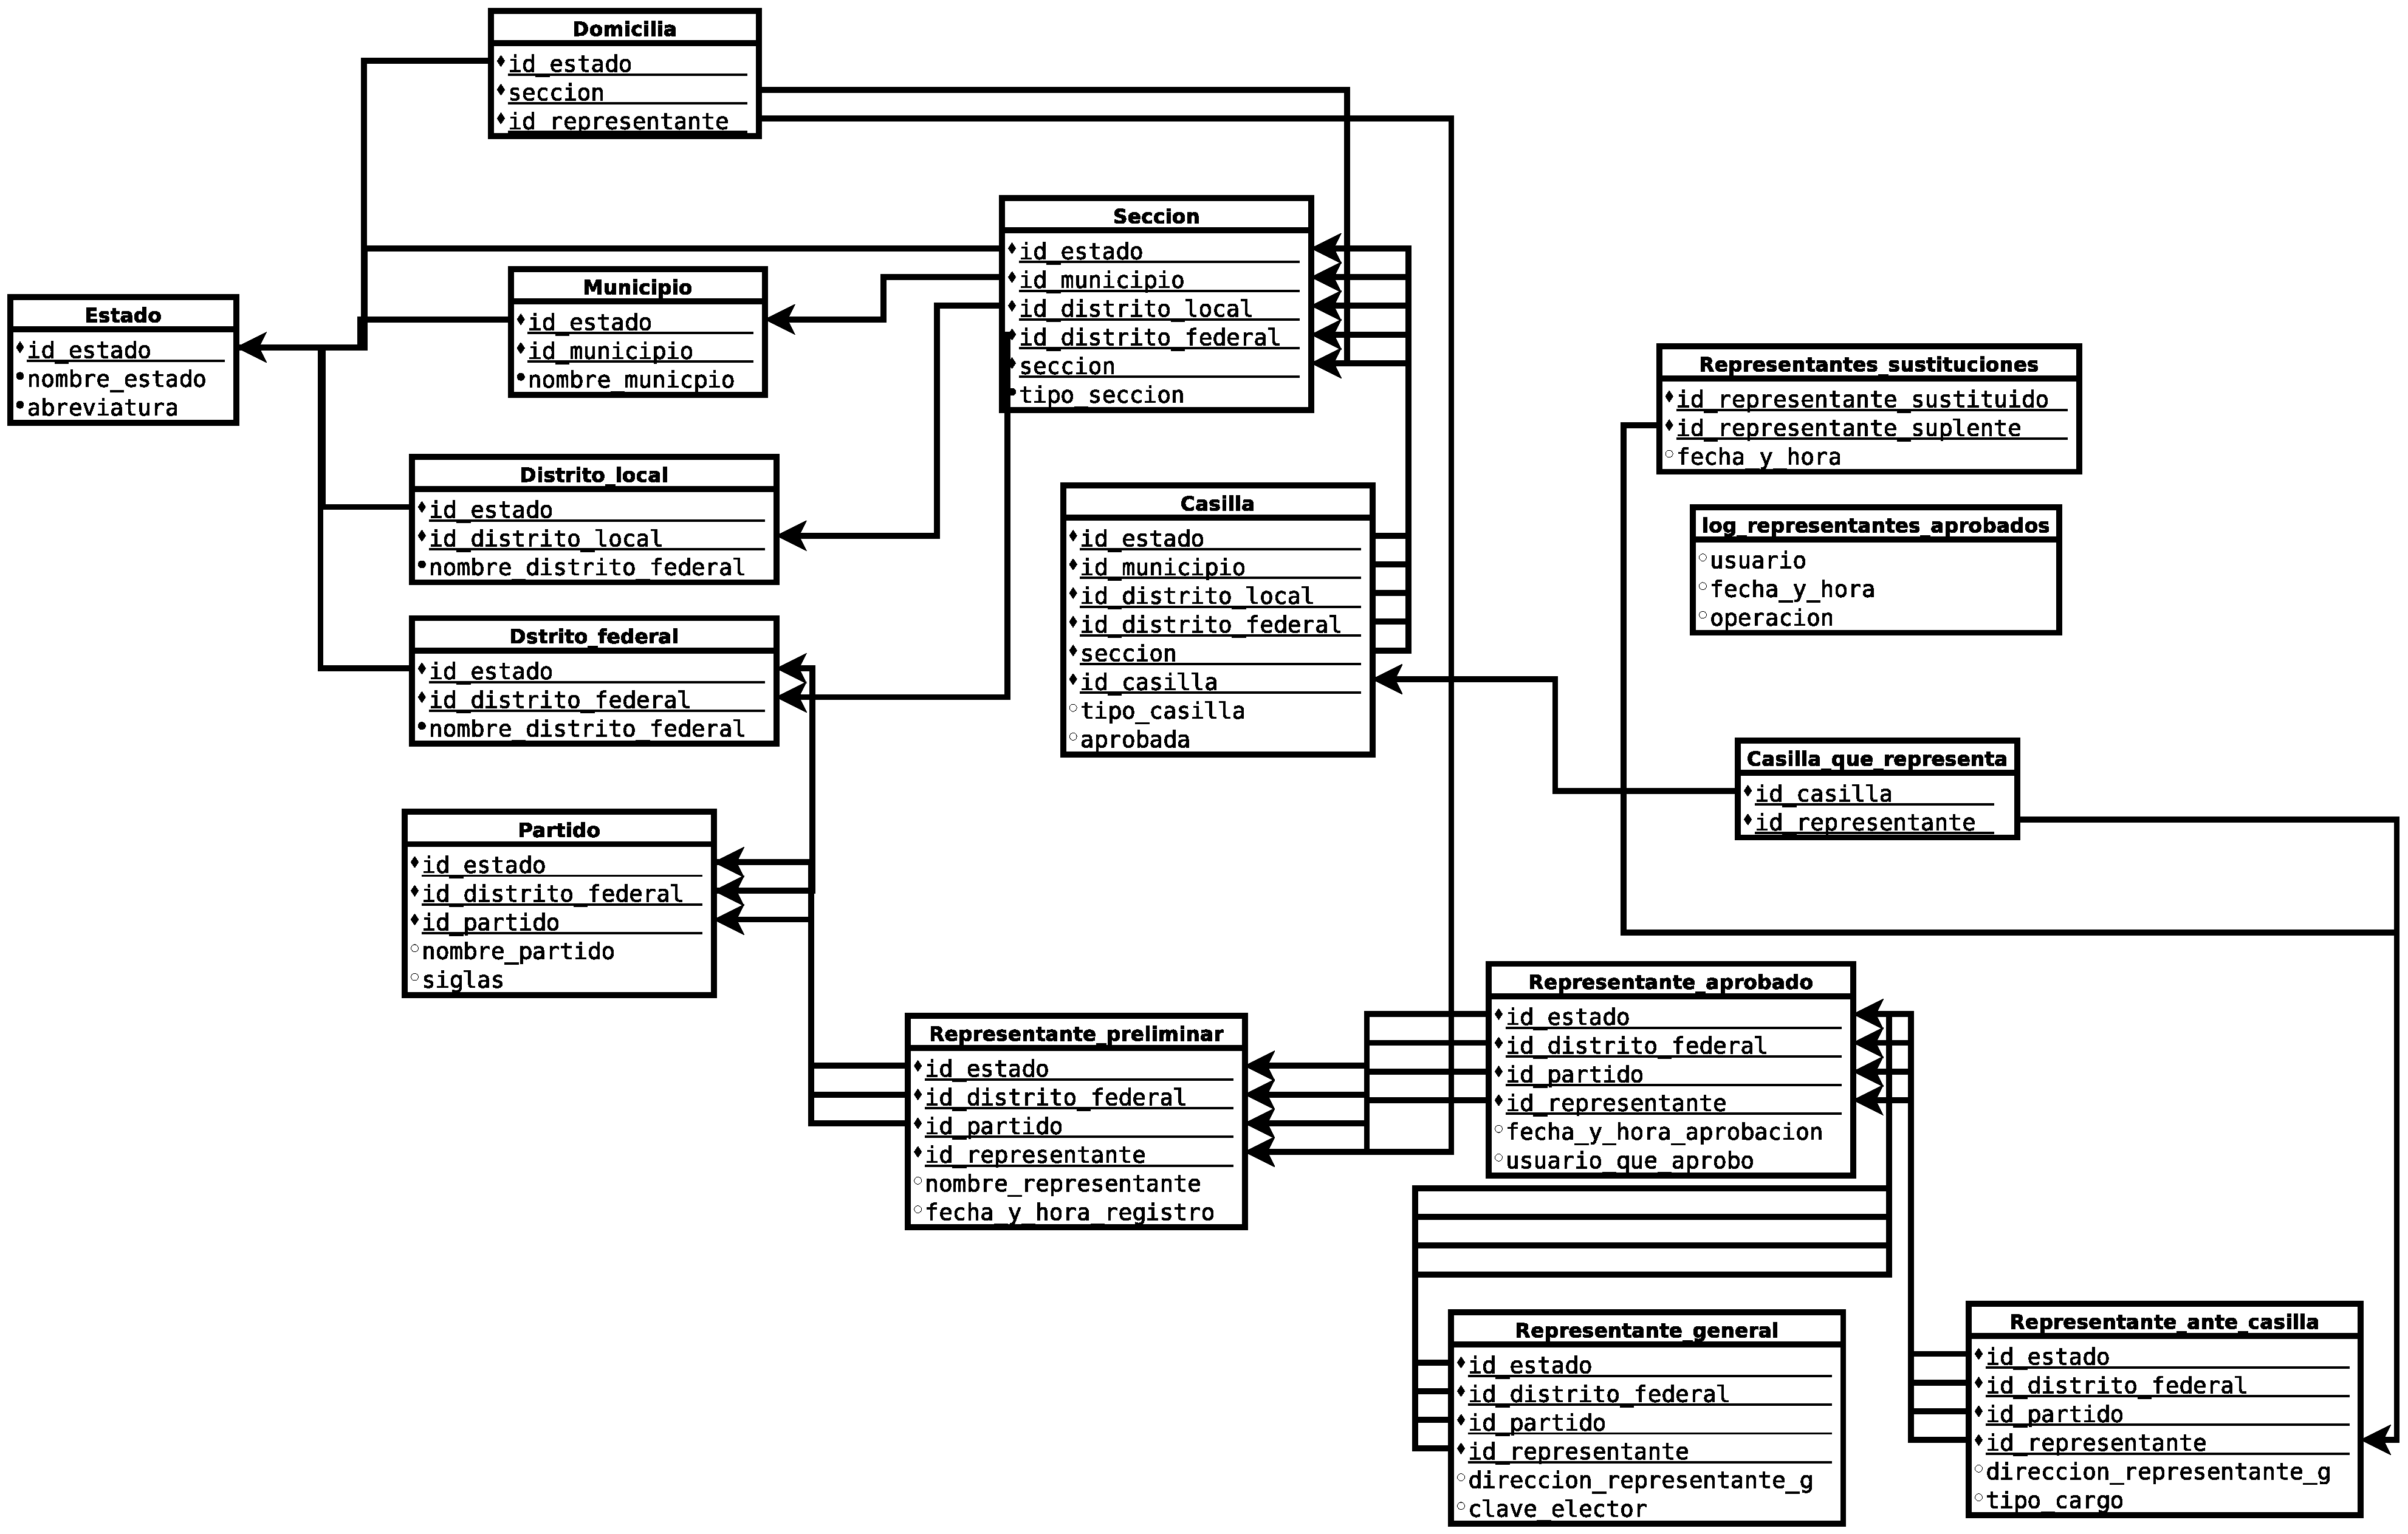
\includegraphics[scale=0.25]{esquema_relacional}\\
\end{document}
